\documentclass[]{MSword}
% Class options:
%-------------------------------
% nobib         - skip bibliography code/ don't include bib
% math          - include math packages and useful math commands
% hidelinks     - hide hyperref colored link boxes
% wordlinks     - link color scheme similar to word


% Preamble code:
%%%%%%%%%%%%%%%%%%%%%%%%%%%%%%%%%%%%%%%%
\usepackage[english]{babel}
\usepackage{csquotes}
\usepackage{lipsum}
\addbibresource{bib/bibliography.bib}

% % Uncomment using "Ctrl + /" (/ on numpad):
% % Customizing headers and footers:
% \fancypagestyle{custom}{%
%     \fancyhf{}% clears the footer and header
%     % Header:
%     \fancyhead[L]{}
%     \fancyhead[C]{}
%     \fancyhead[R]{}
%     % Footer:
%     \fancyfoot[L]{}
%     \fancyfoot[C]{}
%     \fancyfoot[R]{}
%         % Tips:
%         % ----
%         % L: left, C: center, R: right
%         % O: odd pages, E: even pages
%         % ----
%         % Example: \fancyghead[LO,RE]{Text}
%         % will produce "Text" left in the header
%         % on odd pages and right in the header on even pages.
%     % Rules/ lines:
%     \renewcommand{\headrulewidth}{0.4pt}
%     \renewcommand{\footrulewidth}{2pt}
% }
% % Changing the pagestyle:
% \pagestyle{custom}

%%%%%%%%%%%%%%%%%%%%%%%%%%%%%%%%%%%%%%%%

% Preamble information:
%%%%%%%%%%%%%%%%%%%%%%%%%%%%%%%%%%%%%%%%

\title{Background Research}
\author{Ben Wakefield}
\date{February 2023}

%%%%%%%%%%%%%%%%%%%%%%%%%%%%%%%%%%%%%%%%

% The document:
%%%%%%%%%%%%%%%%%%%%%%%%%%%%%%%%%%%%%%%%
\begin{document}

\maketitle
\begin{center}
    Words: \quickwordcount{main}\\ % Word count 
\end{center}

\section{Models for Music Generation}
\par{Jukebox, MuseNet, PerformanceRNN, and Riffusion are all AI music generation models that use deep neural networks. However, they use different types of neural network architectures and techniques to generate music, and have varying levels of usability.}

\subsection*{Jukebox}

\begin{center}
  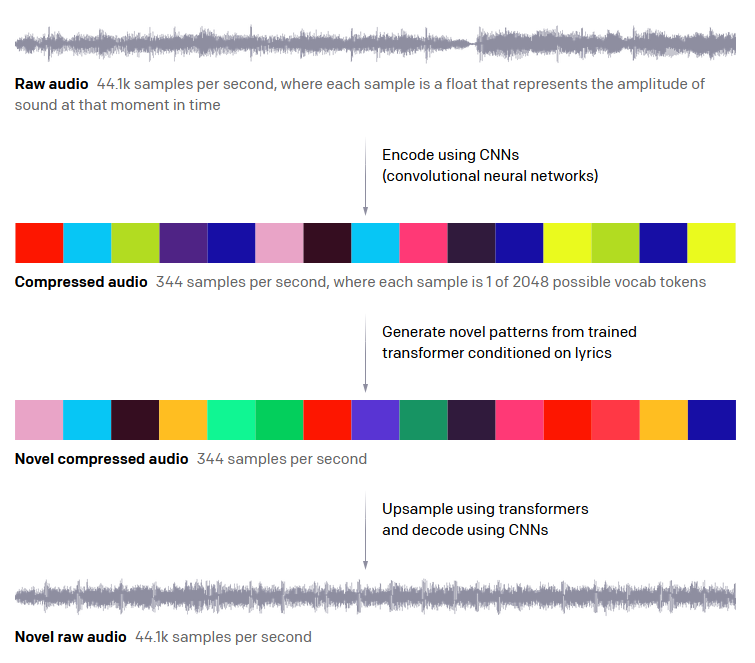
\includegraphics[width=0.5\textwidth]{img/jukebox.png}
\end{center}

\par{OpenAI Jukebox\cite{jukebox} is an AI system developed by OpenAI that uses a combination of deep neural networks and natural language processing to generate music in a variety of styles and genres. The system is based on a large corpus of music that has been preprocessed and organized into a hierarchy of musical concepts, such as scales, chords, and melody lines. When a user inputs a musical prompt, such as a short melody or a genre, the system generates a sequence of musical events that follow the input and are consistent with the hierarchical structure of the music corpus.}

\par{OpenAI Jukebox is trained on a dataset of over a million songs, and its deep neural networks have billions of parameters. The system is capable of generating original compositions in a wide range of styles and genres, from classical and jazz to pop and hip-hop. The generated music can be customized by adjusting parameters such as the tempo, key, and instrumentation.}

\subsection*{MuseNet}

\begin{center}
  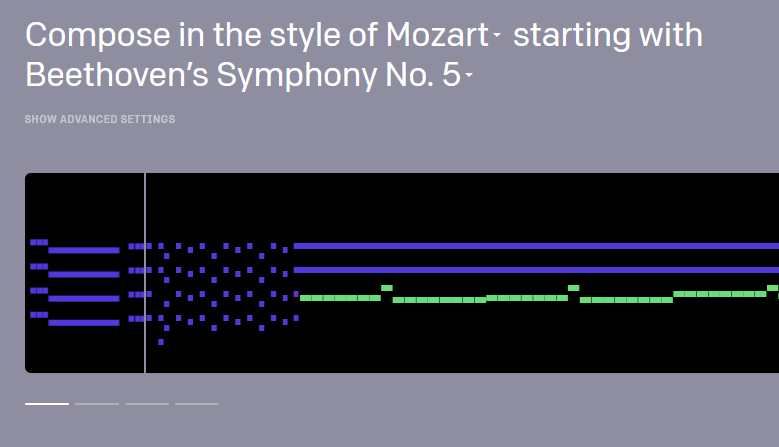
\includegraphics[width=0.5\textwidth]{img/musenet.png}
\end{center}

\par{MuseNet\cite{musenet} is an AI system developed by OpenAI that uses deep neural networks to generate music in a wide range of genres and styles. The system is based on a generative model architecture that uses a combination of hierarchical latent variables and autoregressive models to generate long sequences of musical events. MuseNet is trained on a massive dataset of MIDI files that cover a broad range of musical genres and styles, including classical, jazz, pop, and rock. The system can generate original compositions of varying lengths and complexity, and users can specify parameters such as the genre, tempo, and instrumentation to customize the output.}

\par{One of the key features of MuseNet is its ability to generate music that is both diverse and coherent. The system is able to learn and incorporate complex musical structures and patterns from the training data, enabling it to generate music that is musically consistent and coherent, while also being diverse and unpredictable.}

\subsection*{PerformanceRNN}

\begin{center}
  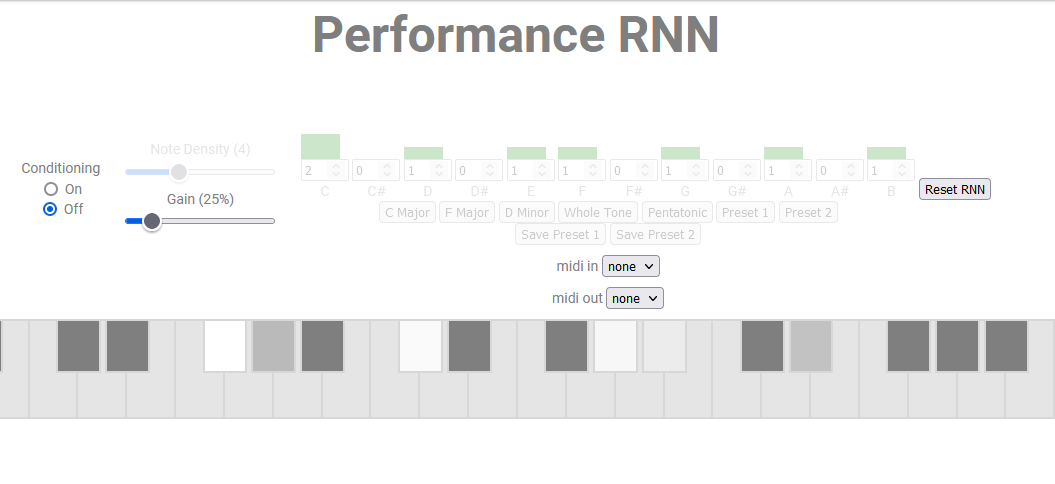
\includegraphics[width=0.5\textwidth]{img/performancernn.png}
\end{center}

\par{PerformanceRNN\cite{performancernn} is a recurrent neural network (RNN) model developed by the Magenta project at Google that is designed to generate expressive and nuanced music performances. Unlike other AI music generation models that focus on generating music notation or MIDI files, PerformanceRNN generates raw audio waveforms that capture the detailed nuances and subtleties of a musical performance, such as the timing, phrasing, and articulation.}

\par{The model is trained on a large dataset of music performances, such as piano recordings and MIDI files, and uses a combination of LSTM (Long Short-Term Memory) and WaveNet architectures to generate high-quality audio waveforms. The system is able to generate performances in a wide range of styles and genres, including classical, jazz, and pop.}

\par{PerformanceRNN is designed to be highly flexible and customizable, allowing users to specify various parameters, such as the style and genre of the music, as well as the level of expressiveness and complexity. The system can also be used for tasks such as music transcription and arrangement, as it is able to analyze and generate complex musical structures and patterns.}

\subsection*{Riffusion}

\begin{center}
  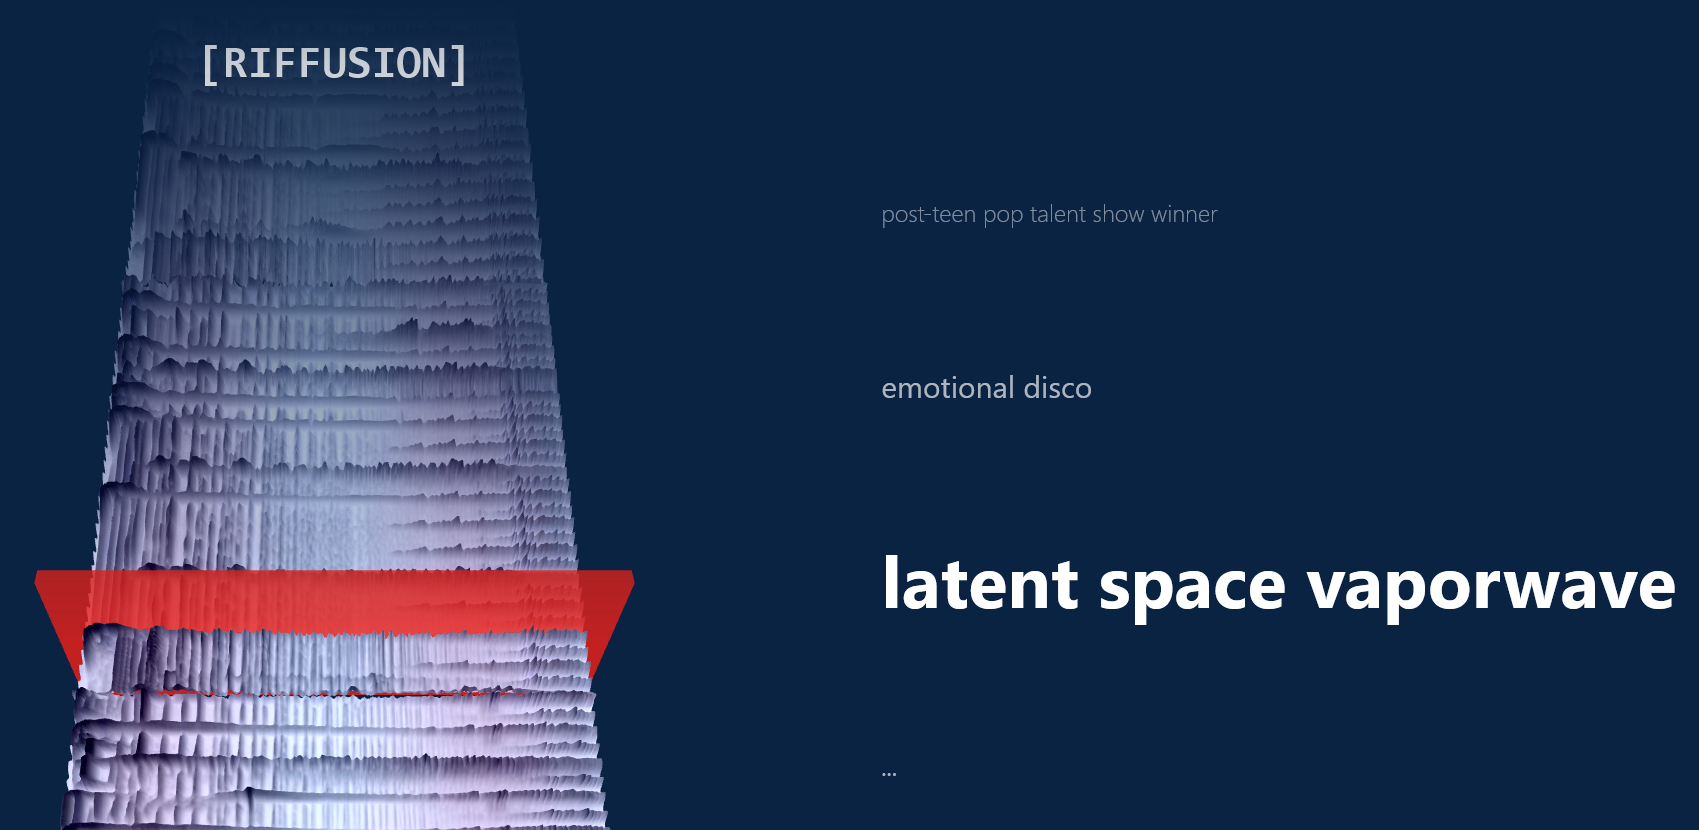
\includegraphics[width=0.5\textwidth]{img/riffusion.png}
\end{center}

\par{Riffusion\cite{riffusion} is an open-source music generation system developed by the Riffusion research group at the University of Montreal. The system uses a combination of deep neural networks and evolutionary algorithms to generate novel and creative musical sequences, such as melodies, chords, and rhythms.}

\par{The system is based on a generative model architecture that uses deep recurrent neural networks (RNNs) to learn the statistical patterns and relationships in a large corpus of MIDI data. The system also employs an evolutionary algorithm to guide the generation process, allowing the model to explore and discover new and creative musical sequences that are not present in the training data.}

\par{One of the unique features of Riffusion is its ability to generate music that is both diverse and coherent. The system can generate complex and intricate musical structures and patterns, while also maintaining a consistent musical style and coherence. The system is also highly customizable, allowing users to specify various parameters such as the style, genre, and complexity of the music.}

\section{Limitations}

\par{The biggest challenge with these models is that they often generate music that is repetitive or lacking in originality. This is because the models tend to learn and replicate common patterns and structures from the training data, which can lead to a lack of novelty in the generated music. Additionally, generating high-quality music requires a significant amount of computational resources, which can be a limiting factor for many users. Training and generating music with these models can be computationally intensive and require specialized hardware such as GPUs or TPUs.}

\par{Furthermore, these models are still in the early stages of development, and there is still much to be learned about how to generate truly creative and expressive music with AI. While these models have made significant progress in generating realistic and coherent music, they still have limitations in terms of their ability to generate truly original and innovative music.}

\par{Lastly, these models typically lack accessibility and generally would not be used in a typical users workflow. They require knowledge of command-line applications, installing dependencies, and creating virtual environments. MuseNet\cite{musenetdemo}, Magenta\cite{performancernndemo}, and Riffusion\cite{riffusiondemo} provide demos for experimenting with the models, but the output is at reduced quality and the UI limits some customization options.}

\section{Improvements}

\par{In essence, this project will focus on a simpler user-interface. The models will also already be fine-tuned to a very specific style in order to yield the best results, without the user having to tediously experiment with parameters and wait for training to take place. Additionally, the interface will allow users to provide feedback to the model, letting them rank results on a quality scale, which will be fed back into the model for continuous improvement.}

\printbibliography

\end{document}

%%%%%%%%%%%%%%%%%%%%%%%%%%%%%%%%%%%%%%%%

% Copyright Remarks:
%--------------------

% Copyright holder: Vebjørn S. Førde, copyright: CC BY 4.0
% Note: The author of this template is also the copyright holder.

% Below is an explanation of the CC BY 4.0. Additional statements/ 
% clarifications made by the author/copyright holder are marked with *.

% YOU ARE FREE TO:
% Share — copy and redistribute the material in any medium or format
% Adapt — remix, transform, and build upon the material
% for any purpose, even commercially.

% UNDER THE FOLLOWING TERMS:
% Attribution* — You must give appropriate credit, provide a link to the license,
% and indicate if changes were made. You may do so in any reasonable manner, but 
% not in any way that suggests the licensor endorses you or your use.

% *Note: 
% Attribution NOT NEEDED for: 
%       - PDF distibution (like sharing your PDF document)
%       - Use of (dummy)text and images provided in the template (obviously)
%       - Distributing parts of the template, and not the template as a whole
% I am not really concerned with being given credit. As long as you do not 
% claim to have made the template yourself in distributing it further, I have
% no complaints.

% No additional restrictions — You may not apply legal terms or technological 
% measures that legally restrict others from doing anything the license permits.

% NOTICES:
% No warranties are given.

% Disclaimer* (added by copyright holder):
% THE SOFTWARE IS PROVIDED "AS IS", WITHOUT WARRANTY OF ANY KIND, EXPRESS OR
% IMPLIED, INCLUDING BUT NOT LIMITED TO THE WARRANTIES OF MERCHANTABILITY,
% FITNESS FOR A PARTICULAR PURPOSE AND NONINFRINGEMENT. IN NO EVENT SHALL THE
% AUTHORS OR COPYRIGHT HOLDERS BE LIABLE FOR ANY CLAIM, DAMAGES OR OTHER
% LIABILITY, WHETHER IN AN ACTION OF CONTRACT, TORT OR OTHERWISE, ARISING FROM,
% OUT OF OR IN CONNECTION WITH THE SOFTWARE OR THE USE OR OTHER DEALINGS IN THE
% SOFTWARE.

% Read more about CC BY 4.0:
% https://creativecommons.org/licenses/by/4.0/